%%%%%%%%%%%%%%%%%%% EJERCICIO 15 %%%%%%

\textbf{Ejemplo 15}\\
Una persona debe pagar  COP  100,000 con vencimiento en 3 meses,  COP  150,000 a 10 meses y
COP  200,000 con vencimiento en un año. Si hace un pago único de  COP  450,000, hallar la fecha en
que debe hacerse, suponga una tasa del 18\% nominal anual mes vencido.
Si consideramos la período focal (pf) en el período mes vencido 12:\\ \\

%\newpage %USAR SOLO SI EL SOLUCIÓN QUEDA SOLO Y ES NECESARIO BAJARLO A LA SIGUIENTE PAGINA
\textbf{Solución.}\\
%La tabla ira centrada
\begin{center}
  \renewcommand{\arraystretch}{1.5}% Margenes de las celdas
  %Creación de la cuadricula de 3 columnas
  \begin{longtable}[H]{|c|c|c|}
    %Creamos una linea horizontal
    \hline
    %Definimos el color de la primera fila
    \rowcolor[HTML]{FFB183}
    %%%%% INICIO ASIGNACIÓN PERíODO FOCAL %%%%%%%
    %%%%%%%%%% INICIO TITULO
    %Lo que se hace aquí es mezclar las 3 columnas en una sola
    \multicolumn{3}{|c|}{\cellcolor[HTML]{FFB183}\textbf{1. Asignación período focal}}                                                                                          \\ \hline
    \multicolumn{3}{|c|}{\textbf{ $pf = \textit{ período focal: 0 pmv} $}}                                                                                                      \\ \hline
    %%%%%%%%%% FIN TITULO
    %%%%% INICIO DECLARACIÓN DE VARIABLES %%%%%%%
    %%%%%%%%%% INICIO TITULO
    %Lo que se hace aquí es mezclar las 3 columnas en una sola
    \multicolumn{3}{|c|}{\cellcolor[HTML]{FFB183}\textbf{2. Declaración de variables}}                                                                                          \\ \hline
    %%%%%%%%%% FIN TITULO
    %%%%%%%%%% INICIO DE MATEMÁTICAS
    %Cada & hace referencia al paso de la siguiente columna

    $j = 18\% \textit{ namv} $                                 & $P_{1} =  COP  100.000  $                                                      & $n_{1} = 9 \textit{ pmv} $    \\
    $i = 1,5\% \textit{ pmv} $                                 & $P_{2} =  COP  150.000  $                                                      & $n_{2} = 2 \textit{ pmv} $    \\
                                                               & $P_{3} =  COP  200.000  $                                                      & $n_{3}= 0 \textit{ pmv}  $    \\
                                                               & $p_{4} =  COP  450.000  $                                                      & $n_{4} = 12-n \textit{ pmv} $ \\ \hline

    %%%%%%%%%% FIN DE MATEMÁTICAS
    %%%%% FIN DECLARACIÓN DE VARIABLES


    %%%%% INICIO FLUJO DE CAJA
    \rowcolor[HTML]{FFB183}
    \multicolumn{3}{|c|}{\cellcolor[HTML]{FFB183}\textbf{3. Diagrama de flujo de caja}}                                                                                         \\ \hline
    %Mezclamos 3 columnas y pondremos el dibujo
    %%%%%%%%%%%%% INSERCIÓN DE LA IMAGEN
    %Deberán descargar las imágenes respectivas del drive y pegarlas en la carpeta
    %n_capitulo/img/ejemplos/1/capitulo1ejemplo1.pdf  (el /1/ es el numero del ejemplo)
    \multicolumn{3}{|c|}{ 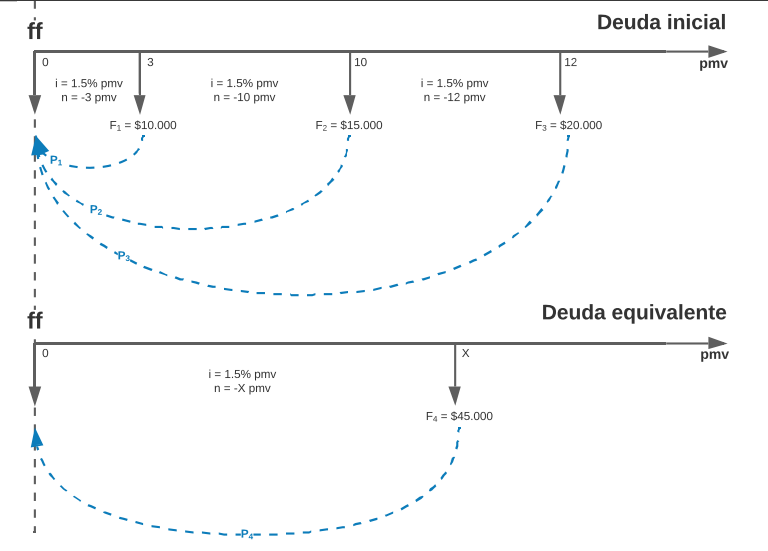
\includegraphics[trim=-5 -5 -5 -5 , scale=0.64]{14/Capitulo2Ejercicio15.pdf} }
    \\ \hline
    %%%%%%%%%%%%% FIN INSERCIÓN DE IMAGEN
    %%%%%FIN FLUJO DE CAJA



    %%%%% INICIO DECLARACIÓN FORMULAS
    %%%%%%%%%%% INICIO TITULO
    \rowcolor[HTML]{FFB183}
    \multicolumn{3}{|c|}{\cellcolor[HTML]{FFB183}\textbf{4. Declaración de fórmulas}}                                                                                           \\ \hline
    %%%%%%%%%%% FIN TITULO
    %%%%%%%%%%% INICIO MATEMÁTICAS

    $P_{1} + P_{2} + P_{3} = P_{4} \textit{ Ecuación de eqv.}$ & \multicolumn{2}{c|}{$P = F(1+i)^(-n) \hspace{0.3cm} \textit{Valor presente}$ }                                 \\
                                                               & \multicolumn{2}{c|}{$F = P(1+i)^n \hspace{0.3cm} \textit{Valor futuro}$   }                                    \\ \hline
    %%%%%%%%%% FIN MATEMÁTICAS
    %%%%%% INICIO DESARROLLO MATEMÁTICO
    \rowcolor[HTML]{FFB183}
    %%%%%%%%%%INICIO TITULO
    \multicolumn{3}{|c|}{\cellcolor[HTML]{FFB183}\textbf{5. Desarrollo matemático}}                                                                                             \\ \hline
    %%%%%%%%%% FIN TITULO
    %%%%%%%%%% INICIO MATEMÁTICAS

    \multicolumn{3}{|C{\linewidth}|}{$  COP  100.000( 1 + 0,015)^(-3) +  COP  150.000( 1 + 0,015)^(-10) +  COP  200.000( 1 + 0,015)^(-12)= COP  450.000( 1 + 0,015)^(-x) $}     \\
    \multicolumn{3}{|C{\linewidth}|}{$ ln(306.090,07391/450.000)= (-x)ln(1,015)  $ }                                                                                            \\ \hline


    %%%%%%%%%% FIN MATEMÁTICAS
    %%%%%% FIN DESARROLLO MATEMÁTICO
    %%%%%% INICIO RESPUESTA
    \rowcolor[HTML]{FFB183}
    %%%%%%%%%%INICIO TITULO
    \multicolumn{3}{|c|}{\cellcolor[HTML]{FFB183}\textbf{6. Respuesta}}                                                                                                         \\ \hline
    %%%%%%%%%% FIN TITULO
    %%%%%%%%%% INICIO RESPUESTA MATEMÁTICA
    \multicolumn{3}{|c|}{

      \begin{minipage}[t][0.07\textheight][c]{0.8\columnwidth}
        $n_{4} = 9,24059 \textit{ pmv} \approx t = 9 \textit{ meses y }  7 \textit{ dias.} $
      \end{minipage}
    }                                                                                                                                                                           \\ \hline


    %%%%%%%%%% FIN MATEMÁTICAS
    %%%%%% FIN RESPUESTA
  \end{longtable}
  %Se crean dos lineas en blanco para que no quede el siguiente texto tan pegado
  %\newline \newline %USARLO SI CREES QUE ES NECESARIO
\end{center}
%%%%%%%%%%%%%%%%%%%%%%%%%%FIN EJERCICIO 15 %%%%%%%%%%%%%%%%%%%%%%%%%%%
